\documentclass[a4paper]{scrartcl}
\usepackage{mathe-blatt}
\usepackage{graphicx}
\usepackage{listings}
\blattnumeins

\begin{document}

\begin{aufgabe}
	\begin{enumerate}[a)]
		\item
			Sei $A^{(k)}$ die Matrix $A$ im $k$-ten Schritt der LR-Zerlegung (also $A^{(k-1)}=R, A^{(0)}=A$).

			Zeige induktiv, dass alle Pivotelemente $a_{k,k}^{(k-1)}$ für $k=1,\dotsc,n-1$ ungleich Null sind, dann existiert nämlich nach dem Algorithmus die LR-Zerlegung für $A$.

			\begin{seg}{Induktionsanfang ($n=1$)}
				$\displaystyle 1 \neq \det(\tilde A_1) = a_{1,1} = a_{1,1}^{(0)}$
			\end{seg}
			\begin{seg}{Induktionsschritt}
				Seien $a_{j,j}^{(j-1)}$ für $j=1,\dotsc,k$ ungleich Null, dann existiert die LR-Zerlegung $\tilde A_{k+1} = \tilde L_{k+1} \tilde R_{k+1}$ für die $(k+1)\times (k+1)$-Matrix $\tilde A_{k+1}$.
				Angenommen, $a_{k+1,k+1}^{(k)} = 0$, dann besitzt $\tilde R_{k+1}$ unten eine Nullzeile und demnach
				\[
					\det(\tilde A_{k+1}) = \det(\tilde L_{k+1}) \cdot \underbrace{\det(\tilde R_{k+1})}_{=0} = 0
				\]
				Ein Widerspruch zu der Vorraussetzung $\det(A_{k+1}) \neq 0$.
				Damit gilt für das Pivotelement: $a_{k+1,k+1}^{(k)} \neq 0$.
			\end{seg}
		\item
			Seien $L_1R_1 = A = L_2R_2$ zwei LR-Zerlegungen von $A$, dann ist
			\[
				L_2^{-1}L_1 = R_2R_1^{-1}
			\]
			Da Dreiecksmatrizen bezüglich der Matrixmultiplikation eine Gruppe bilden, sind die Inversen auch jeweils (linke, bzw. rechte) Dreiecksmatrizen, insbesondere auch das Produkt zweier.
			Es muss sich also eine Diagonalmatrix ergeben: $L_2^{-1}L_1 = R_2R_1^{-1} = D$.
			Da jedoch $L_2^{-1}$ nur Einsen auf der Diagonalen haben kann (verifiziere durch die Matrixmultiplikation $L_2^{-1}L = I$, ergibt sich für $D$ die Einheitsmatrix $I$.
			Damit gilt offensichtlich
			\[
				L_1 = L_2
			\]
	\end{enumerate}
\end{aufgabe}

\begin{aufgabe}~

	Bezeichne das Teilpolynom auf dem Intervall $[k-1,k]$ durch
	\[
		p_k(x) = a_k(x-(k-1))^3 + b_k(x-(k-1))^2 + c_k(x-(k-1)) + d_k
	\]
	Da $s\in C^2$, ist $s$ zweimal stetig differenzierbar.
	Weil $s$ außerhalb von $[-2,2]$ konstant $0$ ist, also $s(x)=s'(x)=s''(x)=0$ für $x\in [a,b]\setminus [-2,2]$, folgt unmittelbar aus der Stetigkeit von $s$ und ihren Ableitungen, dass
	\[
		s(-2) = s'(-2) = s''(-2) = 0 = s(2) = s'(2) = s''(2)
	\]
	Aus obigen Gleichungen ergeben sich schonmal sechs Bedingungen für die Teilpolynome.
	Weitere neun erhält man, da die Polynome jeweils zusammenhängend und glatt an den Stützstellen sein müssen.
	Durch den Punkt $s(0) = 1$ erhält dann die letzte.

	Diese 16 Gleichungen bilden ein Gleichungssystem mit 16 Unbekannten, das eindeutig lösbar ist (betrachte die Determinante)
	\setcounter{MaxMatrixCols}{16}
	\[
		\begin{pmatrix}[rrrrrrrrrrrrrrrr]
			0 & 0 & 0 & 1 & 0 & 0 & 0 & 0 & 0 & 0 & 0 & 0 & 0 & 0 & 0 & 0 \\
			0 & 0 & 1 & 0 & 0 & 0 & 0 & 0 & 0 & 0 & 0 & 0 & 0 & 0 & 0 & 0 \\
			0 & 2 & 0 & 0 & 0 & 0 & 0 & 0 & 0 & 0 & 0 & 0 & 0 & 0 & 0 & 0 \\
			0 & 0 & 0 & 0 & 0 & 0 & 0 & 0 & 0 & 0 & 0 & 0 & 1 & 1 & 1 & 1 \\
			0 & 0 & 0 & 0 & 0 & 0 & 0 & 0 & 0 & 0 & 0 & 0 & 3 & 2 & 1 & 0 \\
			0 & 0 & 0 & 0 & 0 & 0 & 0 & 0 & 0 & 0 & 0 & 0 & 6 & 2 & 0 & 0 \\
			0 & 0 & 0 & 0 & 1 & 1 & 1 & 1 & 0 & 0 & 0 & 0 & 0 & 0 & 0 & 0 \\
			1 & 1 & 1 & 1 & 0 & 0 & 0 &-1 & 0 & 0 & 0 & 0 & 0 & 0 & 0 & 0 \\
			0 & 0 & 0 & 0 & 1 & 1 & 1 & 1 & 0 & 0 & 0 &-1 & 0 & 0 & 0 & 0 \\
			0 & 0 & 0 & 0 & 0 & 0 & 0 & 0 & 1 & 1 & 1 & 1 & 0 & 0 & 0 &-1 \\
			3 & 2 & 1 & 0 & 0 & 0 &-1 & 0 & 0 & 0 & 0 & 0 & 0 & 0 & 0 & 0 \\
			0 & 0 & 0 & 0 & 3 & 2 & 1 & 0 & 0 & 0 &-1 & 0 & 0 & 0 & 0 & 0 \\
			0 & 0 & 0 & 0 & 0 & 0 & 0 & 0 & 3 & 2 & 1 & 0 & 0 & 0 &-1 & 0 \\
			6 & 2 & 0 & 0 & 0 &-2 & 0 & 0 & 0 & 0 & 0 & 0 & 0 & 0 & 0 & 0 \\
			0 & 0 & 0 & 0 & 6 & 2 & 0 & 0 & 0 &-2 & 0 & 0 & 0 & 0 & 0 & 0 \\
			0 & 0 & 0 & 0 & 0 & 0 & 0 & 0 & 6 & 2 & 0 & 0 & 0 &-2 & 0 & 0 \\
		\end{pmatrix}
		x =
		\begin{pmatrix}
			0 \\ 0 \\ 0 \\ 0 \\ 0 \\ 0 \\ 1 \\ 0 \\ 0 \\ 0 \\ 0 \\ 0 \\ 0 \\ 0 \\ 0 \\ 0
		\end{pmatrix}
	\]
	(die Koeffizienten sind folgendermaßen sortiert: $a_{-1}, b_{-1}, c_{-1}, d_{-1}, a_0, b_0, \dotsc, c_2, d_2$)

	Damit sind die Teilpolynome durch die Lösung des Gleichungssystems eindeutig bestimmt als
	\begin{align*}
		p_{-1}(x) &= \f 14 (x+2)^3 \\
		p_{0}(x) &= -\f 34 (x+1)^3 + \f 34 (x+1)^2 + \f 34 (x+1) + \f 14 \\
		p_{1}(x) &= \f 34 x^3 - \f 32 x^2 + 1 \\
		p_{2}(x) &= -\f 14 (x-1)^3 + \f 34 (x-1)^2 - \f 34 (x-1) + \f 14 \\
	\end{align*}
	Also ist auch der gesamte Spline eindeutig bestimmt.
\end{aufgabe}

\begin{aufgabe}
	\begin{enumerate}[a)]
		\item
			\begin{enumerate}[i)]
				\item
					Es ist $f''(x) = 6x-2$ und damit $f''(0) = -2 \neq 0$, also ist die Randbedingung für natürliche Splines nicht erfüllt und $f\not\in V$.
				\item
					Die Teilpolynome sind durch $f(x)$ wohldefiniert und offensichtlich in $C^2$.
					Außerdem $f''(x) = 6x-12 - 6(x-2)$ und damit
					\begin{align*}
						f''(0) = 0, \qquad	f''(2) = 0
					\end{align*}
					also ist $f\in V$.
				\item
					Es gilt für die Teilpolynome $p_1,p_2$:
					\begin{alignat*}{3}
						p_1(x) &= -\f 12 x^2 & \qquad p_1'(x) &= -\f 32 x^2 & \qquad p_1''(x) &= -3x \\
						p_2(x) &= (x-1)^3 - \f 12 x^3&  \qquad p_2'(x) &= 3(x-1)^2 - \f 32 x^2 & \qquad p_2''(x) &= 6(x-1) -3x
					\end{alignat*}
					Man sieht leicht, dass die beiden Polynome zusammenhängend und glatt an der Stelle $x_1=1$ sind.
					Auch die Randbedingung ist erfüllt:
					\[
						p_1''(0) = 0, \qquad p_2''(2) = 6 - 6 = 0
					\]
					Damit ist $f\in V$.
				\item
					Für das zweite Teilpolynom gilt 
					\begin{align*}
						p_2(x) &= -3(x-2)^2+3 \\
						p_2'(x) &= -6(x-2) \\
						p_2''(x) &= -6 \neq 0
					\end{align*}
					Also ist die Randbedingung $s(2)=0$ für natürliche Splines nicht erfüllt und $f\not\in V$.
			\end{enumerate}
		\item
			Aus der Matrixdarstellung für die $M_k$ ergibt sich sofort
			\[
				4 = 2(h_1+h_2) M_1 = 6(f_2 - f_1) - 6(f_1 - f_0) = 36 \implies M_1 = 9
			\]
			Die Randbedingungen legen außerdem fest: $M_0=0$ und $M_2=0$.
			Damit sind die Koeffizienten der Teilpolynome eindeutig bestimmt:
			\begin{align*}
				a_1 &= \f {M_1-M_0}{6h_1} = \f 32 \\
				b_1 &= \f {M_0}2 = 0 \\
				c_1 &= \f {f_1 - f_0}{h_1} - h_1\l(\f {M_1}6 + \f {M_0}3\r) = 1 - \f 32 = -\f 12 \\
				d_1 &= f_0 = 0 \\
				a_2 &= \f {M_2-M_1}{6h_2} = -\f 32 \\
				b_2 &= \f {M_1}2 = \f 92 \\
				c_2 &= \f {f_2 - f_1}{h_2} - h_2\l(\f {M_2}6 + \f {M_1}3\r) = 7 - 3 = 4 \\
				d_2 &= f_2 = 1
			\end{align*}
			Damit sind die Teilpolynome des Splines gegeben durch
			\begin{align*}
				p_1(x) &= \f 32 x^3 - \f 12 x \\
				p_2(x) &= -\f 32 (x-1)^3 + \f 92 (x-1)^2 + 4(x-1) + 1
			\end{align*}
			Wird die Randbedingung ersetzt, dann gilt
			\begin{align*}
				\tilde M_0 &= f''(0) = 0 \\
				\tilde M_2 &= f''(2) = 12
			\end{align*}
			berechne die sich ändernden Koeffizienten neu:
			\begin{align*}
				\tilde a_2 &= \f {\tilde M_2-\tilde M_1}{6h_2} = 2 - \f 32 =  \f 12 \\
				\tilde c_2 &= \f {f_2 - f_1}{h_2} - h_2\l(\f {\tilde M_2}6 + \f {\tilde M_1}3\r) = 7 - 5 = 2 \\
			\end{align*}
			Die neuen Teilpolynome ergeben sich durch die neuen Koeffizienten:
			\begin{align*}
				p_1(x) = \tilde p_1(x) &= \f 32 x^3 - \f 12 x \\
				\tilde p_2(x) &= \f 12 (x-1)^3 + \f 92 (x-1)^2 + 2(x-1) + 1
			\end{align*}
	\end{enumerate}
\end{aufgabe}

\begin{aufgabe}
	\begin{enumerate}[a)]
		\item
			Die eindimensionale FastFourierTransformation:
			\begin{lstlisting}[language=matlab]
% Stephan Hilb, 2706616
function c = ff1d (f)
	N = length(f);
	if (N == 1)
		c = f;
		return;
	end

	D_N2 = diag( exp( (0:-1:-(N/2 - 1)) * i * 2 * pi / N) );

	c_even = ff1d(f(1 : 2 : end));
	c_odd = ff1d(f(2 : 2 : end));

	tmp = D_N2 * c_odd;

	c = zeros(N,1);
	c(1 : N/2) = 0.5 * (c_even + tmp);
	c(N/2 + 1 : N) = 0.5 * (c_even - tmp);
end
			\end{lstlisting}
		\item
			Die zweidimensionale FastFourierTransformation:
			\begin{lstlisting}[language=matlab]
% Stephan Hilb, 2706616
function C = ff2d (F)
	N = length(F);
	for j = 1:N
		C_1(:,j) = ff1d(F(:,j));
	end
	C_2 = transpose(C_1);
	for j = 1:N
		C_3(:,j) = ff1d(C_2(:,j));
	end
	C = transpose(C_3);
end
			\end{lstlisting}
		\newpage
		\item
			Der Aufruf zur Bildfilterung:
			\begin{lstlisting}[language=matlab]
% Stephan Hilb, 2706616
D = double(imread('Bild.png'));
N = length(D);

figure(1), imshow(uint8(real(D)));

% Fast Fourier Transformation
C = ff2d(D);
%C = fft2(D); % schnellere Matlabfunktion zum Testen

% Frequenzen rausfiltern
C(40:210,:) = 0;
C(:,40:210) = 0;

% Inverse Fast Fourier Transformation
D = N*N * conj(ff2d(conj(C)));
%D = ifft2(C); % schnellere Matlabfunktion zum Testen

figure(2), imshow(uint8(real(D)));
			\end{lstlisting}

		\begin{figure*}[h]
			\centering
			\caption{Ursprungsbild links, transformiertes rechts}
			\begin{tabular}{cc}
				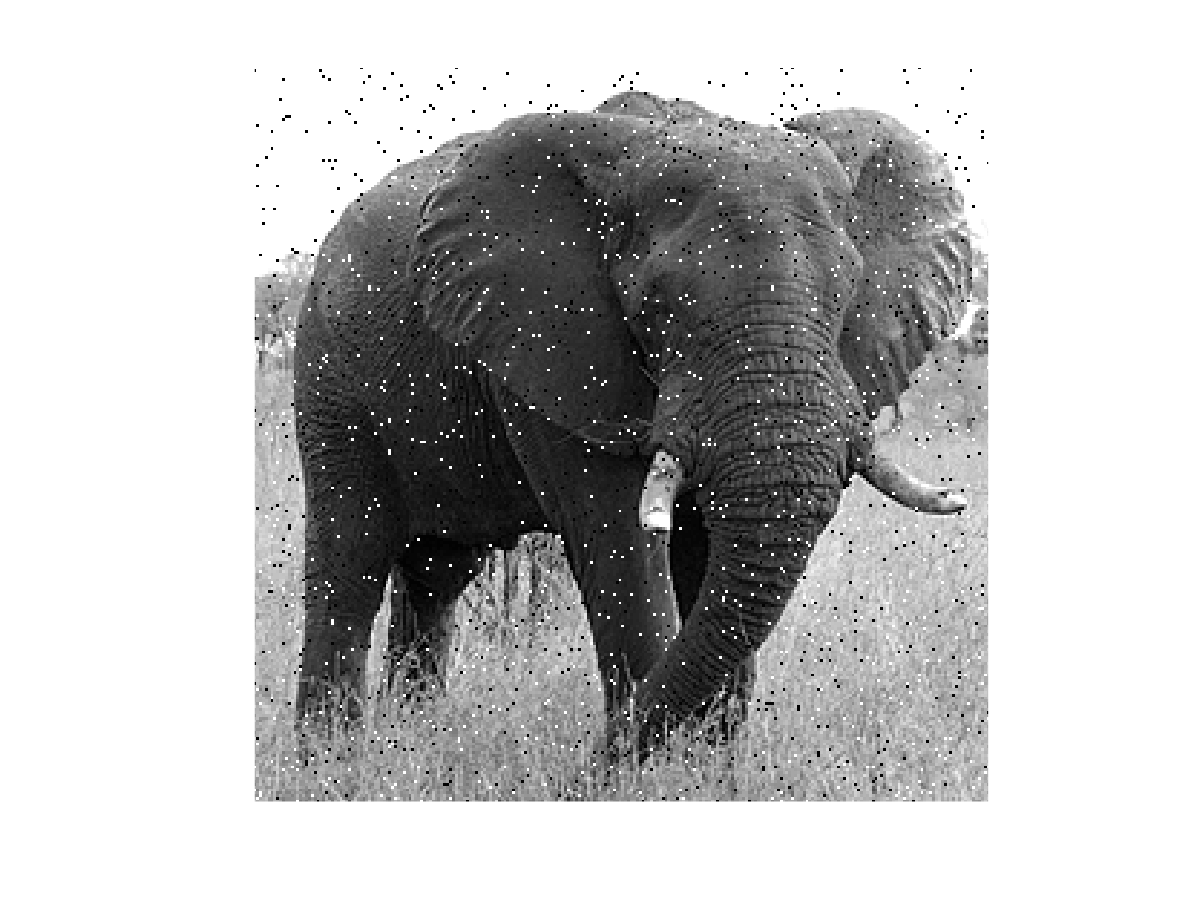
\includegraphics[scale=0.3]{num1_4_4/num1_4_4_1.png}&
				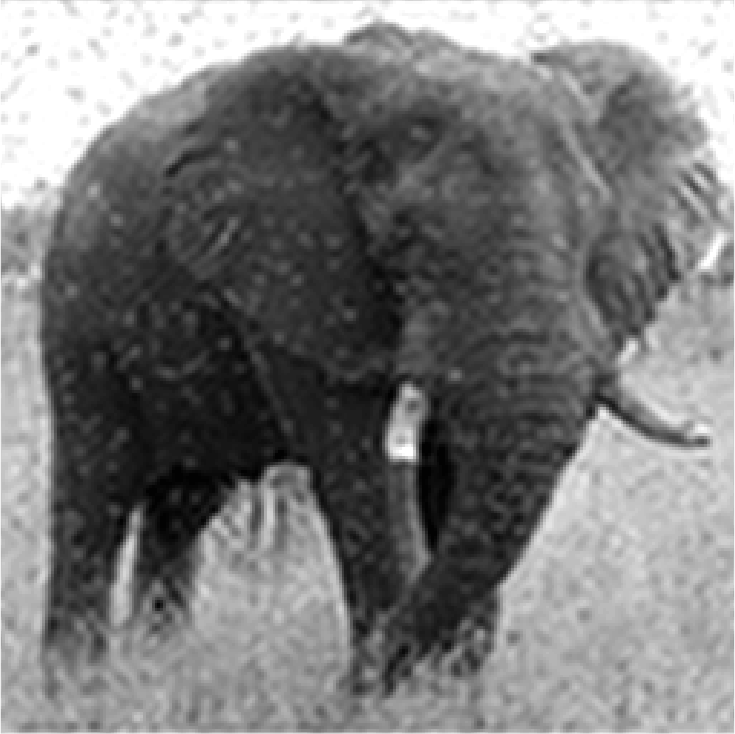
\includegraphics[scale=0.3]{num1_4_4/num1_4_4_2.png}
			\end{tabular}
		\end{figure*}
	\end{enumerate}
\end{aufgabe}


\end{document}
